\documentclass{examen}

\begin{document}
\modulo{Lenguajes de marcas -- PARTE ESCRITA}


\pregunta{En el siguiente XML se han cometido algunos errores. Explica cuales son}{1}
\begin{verbatim}
<!DOCTYPE pedido>
<xml version="1.0" encoding="ISO-8859-2" standalone="true">
<pedido>
   <libro>
     <titulo>Don Quijote</titulo>
     <autor>Miguel de Cervantes</titulo>
   </libro>
   <PAGADO/>
</pedido_>
<pedido_>
   <libro>
     <titulo>Poeta en Nueva York</titulo>
     <autor>Federico Garcia Lorca</titulo>
   </libro>
</pedido>
\end{verbatim}

\pregunta{Elabora una p�gina web que contenga el formulario siguiente:}{4}
\begin{itemize}

\item{    Observa que primero hay dos controles, uno para introducir el login (que es texto) y otro para introducir la clave.}
\item{    El usuario puede elegir una y solo una de dos opciones "Conservar la sesi�n" y "No conservar la sesi�n".}
\item{    El usuario puede elegir 0, 1 o las dos opciones "Iniciar adem�s en servidor X".}
\item{    Hay una lista desplegable con tres opciones, que puedes ver en la captura adjunta.}
\item{ Por favor, recuerda que debes usar HTML v�lido. Comprueba todas las etiquetas.}

 
\end{itemize}
\begin{figure}
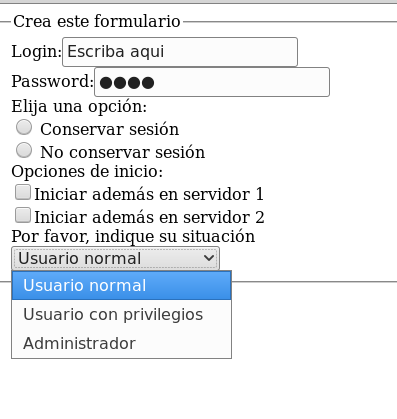
\includegraphics[scale=0.7]{examen-img/foto_formulario_14.png}
\end{figure}
\end{document}

